\documentclass{article}
\usepackage[margin=0.9cm]{geometry}
\usepackage{tikz}
\usetikzlibrary{arrows.meta,positioning,shapes.geometric,calc}

\pagestyle{empty}

\newcommand{\colw}{8.6cm}
\newcommand{\colnarrow}{8.2cm}

\begin{document}

%% ── Figure 1: Offline PC pipeline ─────────────────────────────────────────
\noindent\resizebox{\colw}{!}{%
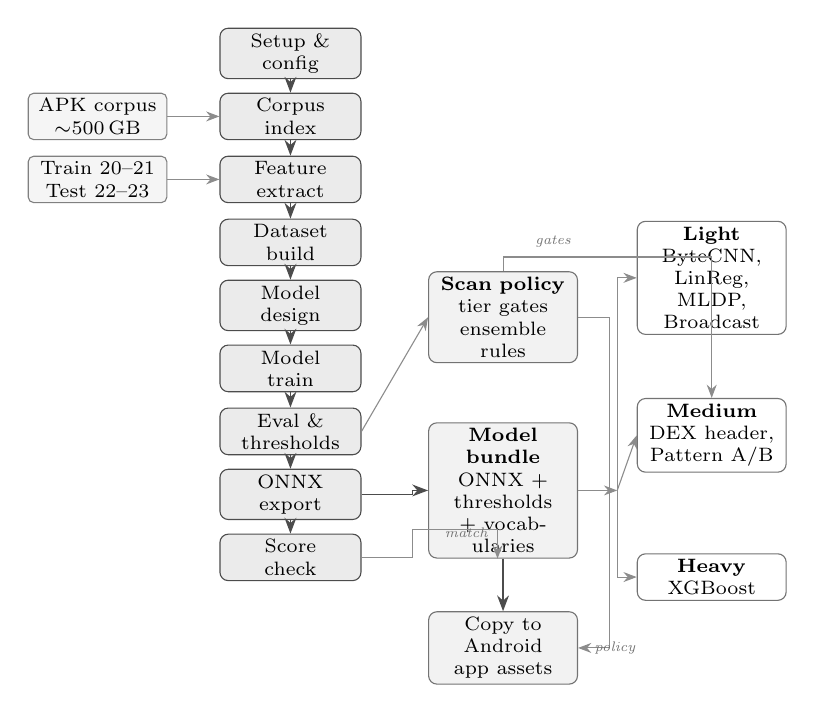
\begin{tikzpicture}[
	font=\scriptsize,
	>=Stealth,
	phase/.style={
		rectangle, rounded corners=3pt,
		draw=black!70, fill=black!8,
		text width=1.65cm, align=center,
		minimum height=0.56cm, inner sep=2pt
	},
	tierbox/.style={
		rectangle, rounded corners=3pt,
		draw=black!55, fill=white,
		text width=1.75cm, align=center,
		minimum height=0.52cm, inner sep=2pt
	},
	side/.style={
		rectangle, rounded corners=2pt,
		draw=black!50, fill=black!4,
		text width=1.62cm, align=center,
		minimum height=0.48cm, inner sep=2pt
	},
	mid/.style={
		rectangle, rounded corners=3pt,
		draw=black!55, fill=black!5,
		text width=1.75cm, align=center,
		minimum height=0.52cm, inner sep=2pt
	},
	arr/.style={->, semithick, black!70},
	sarr/.style={->, thin, black!45},
	lbl/.style={font=\tiny\itshape, black!55}
]

% Spine x=0
\node[phase] (setup)  at (0,  0.00) {Setup \&\\config};
\node[phase] (index)  at (0, -0.80) {Corpus\\index};
\node[phase] (feat)   at (0, -1.60) {Feature\\extract};
\node[phase] (loader) at (0, -2.40) {Dataset\\build};
\node[phase] (arch)   at (0, -3.20) {Model\\design};
\node[phase] (train)  at (0, -4.00) {Model\\train};
\node[phase] (eval)   at (0, -4.80) {Eval \&\\thresholds};
\node[phase] (export) at (0, -5.60) {ONNX\\export};
\node[phase] (verify) at (0, -6.40) {Score\\check};

\foreach \a/\b in {setup/index,index/feat,feat/loader,loader/arch,arch/train,train/eval,eval/export,export/verify}
	\draw[arr] (\a) -- (\b);

% Left inputs
\node[side] (corpus) at (-2.45, -0.80) {APK corpus\\$\sim$500\,GB};
\node[side] (split)  at (-2.45, -1.60) {Train 20--21\\Test 22--23};
\draw[sarr] (corpus.east) -- (index.west);
\draw[sarr] (split.east)  -- (feat.west);

% Middle column x=2.7 — stacked with clear gaps
\node[mid] (policy) at (2.70, -3.35) {
	\textbf{Scan policy}\\
	tier gates\\
	ensemble rules
};
\node[mid, minimum height=0.62cm] (bundle) at (2.70, -5.55) {
	\textbf{Model bundle}\\
	ONNX + thresholds\\
	+ vocabularies
};
\node[mid] (phone) at (2.70, -7.55) {
	Copy to\\Android\\app assets
};

\draw[sarr] (eval.east) -- (policy.west);

% Corridor x=1.55 for spine→bundle arrows (below policy box)
\draw[arr]
	(export.east) -- (1.55, -5.60) -- (1.55, -5.55) -- (bundle.west);
\draw[sarr]
	(verify.east) -- (1.55, -6.40) -- (1.55, -6.05) -| ([xshift=-2pt]bundle.south)
	node[pos=0.55, left, lbl] {match};

\draw[arr] (bundle.south) -- (phone.north);
\draw[sarr]
	(policy.east) -- (4.05, -3.35) -- (4.05, -7.55) -- (phone.east)
	node[pos=0.78, right, lbl] {policy};

% Right column x=5.35 — tier groups
\node[tierbox] (tlight) at (5.35, -2.85) {
	\textbf{Light}\\
	ByteCNN, LinReg,\\
	MLDP, Broadcast
};
\node[tierbox] (tmed) at (5.35, -4.85) {
	\textbf{Medium}\\
	DEX header,\\
	Pattern A/B
};
\node[tierbox] (theavy) at (5.35, -6.65) {
	\textbf{Heavy}\\
	XGBoost
};

% Bus x=4.15 — only horizontal/vertical in open space
\coordinate (bus) at (4.15, -5.55);
\draw[sarr] (bundle.east) -- (bus);
\draw[sarr] (bus) |- (tlight.west);
\draw[sarr] (bus) -- (tmed.west);
\draw[sarr] (bus) |- (theavy.west);

\draw[sarr]
	(policy.north) -- ++(0,0.18) -| (tmed.north)
	node[pos=0.12, above, lbl] {gates};

\end{tikzpicture}%
}

\newpage

%% ── Figure 2: On-device application flow ──────────────────────────────────
\noindent\resizebox{\colnarrow}{!}{%
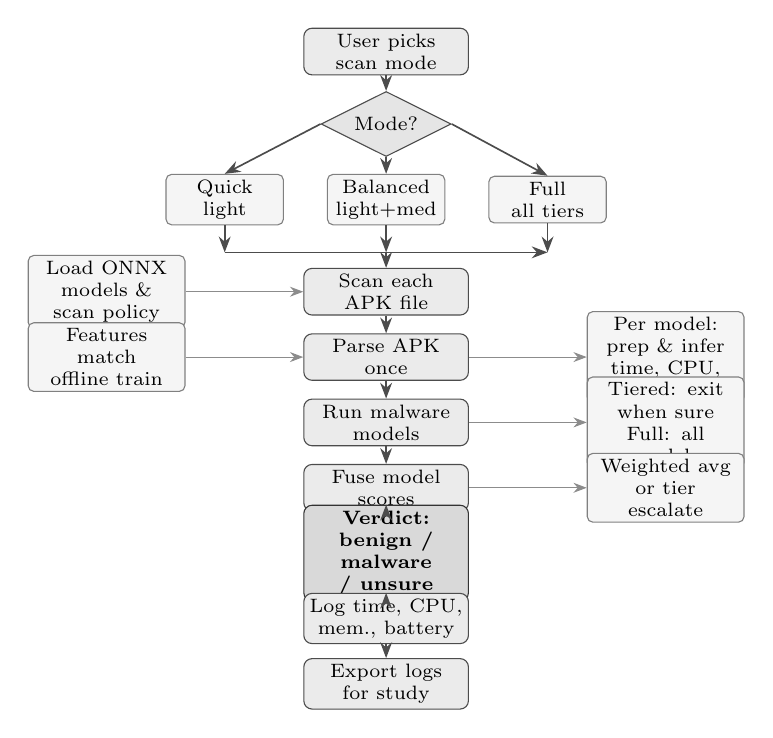
\begin{tikzpicture}[
	font=\scriptsize,
	>=Stealth,
	main/.style={
		rectangle, rounded corners=3pt,
		draw=black!70, fill=black!8,
		text width=1.95cm, align=center,
		minimum height=0.56cm, inner sep=2pt
	},
	decision/.style={
		diamond, aspect=2,
		draw=black!70, fill=black!10,
		text width=1.1cm, align=center,
		inner sep=1pt
	},
	verdict/.style={
		rectangle, rounded corners=3pt,
		draw=black!80, fill=black!15,
		text width=1.95cm, align=center,
		minimum height=0.52cm, inner sep=2pt,
		font=\scriptsize\bfseries
	},
	side/.style={
		rectangle, rounded corners=2pt,
		draw=black!50, fill=black!4,
		text width=1.85cm, align=center,
		minimum height=0.48cm, inner sep=2pt
	},
	arr/.style={->, semithick, black!70},
	sarr/.style={->, thin, black!45}
]

% Centre spine x=0
\node[main] (ui) at (0, 0.00) {User picks\\scan mode};
\node[decision] (depth) at (0, -0.92) {Mode?};

\node[side, text width=1.35cm] (dq) at (-2.05, -1.88) {Quick\\light};
\node[side, text width=1.35cm] (db) at ( 0.00, -1.88) {Balanced\\light+med};
\node[side, text width=1.35cm] (df) at ( 2.05, -1.88) {Full\\all tiers};

\draw[arr] (ui) -- (depth);
\draw[arr] (depth.west) -- (dq.north);
\draw[arr] (depth.south) -- (db.north);
\draw[arr] (depth.east) -- (df.north);

\node[main] (scan)  at (0, -3.05) {Scan each\\APK file};
\node[main] (parse) at (0, -3.88) {Parse APK\\once};
\node[main] (run)   at (0, -4.71) {Run malware\\models};
\node[main] (fuse)  at (0, -5.54) {Fuse model\\scores};
\node[verdict] (verd) at (0, -6.37) {Verdict:\\benign / malware / unsure};
\node[main] (log)   at (0, -7.20) {Log time, CPU,\\mem., battery};
\node[main] (pull)  at (0, -8.03) {Export logs\\for study};

% Merge bus y=-2.55 (clear gap below mode boxes)
\draw[arr] (dq.south) -- (-2.05, -2.55);
\draw[arr] (db.south) -- ( 0.00, -2.55);
\draw[arr] (df.south) -- ( 2.05, -2.55);
\draw[arr] (-2.05, -2.55) -- (2.05, -2.55);
\draw[arr] (0, -2.55) -- (scan.north);

\draw[arr] (scan) -- (parse);
\draw[arr] (parse) -- (run);
\draw[arr] (run) -- (fuse);
\draw[arr] (fuse) -- (verd);
\draw[arr] (verd) -- (log);
\draw[arr] (log) -- (pull);

% Left annotations x=-3.55
\node[side] (models) at (-3.55, -3.05) {
	Load ONNX\\models \&\\scan policy
};
\node[side] (extract) at (-3.55, -3.88) {
	Features match\\offline train
};

\draw[sarr] (models.east) -- (-1.15, -3.05) -- (scan.west);
\draw[sarr] (extract.east) -- (parse.west);

% Right annotations x=3.55 — vertically separated
\node[side] (metrics) at (3.55, -3.88) {
	Per model:\\prep \& infer\\time, CPU, RAM
};
\node[side] (modes) at (3.55, -4.71) {
	Tiered: exit\\when sure\\
	Full: all models
};
\node[side] (pol) at (3.55, -5.54) {
	Weighted avg\\or tier\\escalate
};

\draw[sarr] (parse.east) -- (1.15, -3.88) -- (metrics.west);
\draw[sarr] (run.east) -- (modes.west);
\draw[sarr] (fuse.east) -- (pol.west);

\end{tikzpicture}%
}

\end{document}
